
\section{Making synthetic seismograms}
\label{sect:synt-seismogram}

\index{Synthetic seismograms} 
\index{BOUCH}BOUCH and \index{BOUSEI}BOUSEI, HERRMANN and HERRSEI and WKBJ are all programs which is used for generating synthetic seismograms.\index{WKBJ} 

The full wave modeling programs are written by Bouchon and \index{Herrmann}Herrmann, and for WKBJ, Chapman and Valerie Maupin. Valerie Maupin has integrated WKBJ for SEISAN and written the routines that makes it possible to use specific phases. She has also made many improvements in the original installation of BOUCH and HERRMANN and written a large part of this chapter.   

Bouchon: \newline
The Bouchon program is somewhat modified for SEISAN. The theory, which is quite straight forward, is given in a series of papers (e.g. \citet{bouchon1981}). It is based on a discrete wave number representation of the wave fields. Basically, the source is repeated periodically in space, so that integration over the k-domain is replaced by a series. This implies that the periodicity of the source, L (in km), should be large enough so that the information from fictitious sources does not arrive during the time interval of interest. Roughly r $<$ L/2,  sqrt((L-r)**2+Z**2) $>$ Vp*t where r is the epicentral distance and Vp is the highest P-wave velocity of the model, t is the travel time and Z the hypocentral depth. Only layered (horizontal, parallel) earth model is used. The earthquake source cannot be in the bottom layer or at the surface. 

There are 2 programs, BOUCH and BOUSEI. BOUCH computes the frequency response given the model, the source depth, the focal mechanism, the receiver locations and the orientations of the two horizontal components. BOUSEI takes the output file from BOUCH, multiplies it by the source spectrum and uses an FFT to get the synthetic ground motion (displacement, velocity or acceleration). The user must provide the source function (see below) and the original waveform files must be available in WAV or working directory if a file containing both real and synthetic signal is to be generated. Otherwise, only synthetic data will be seen in the output file. 

Herrmann: \newline
The Herrmann programs HERRMANN and HERSEI \index{HERSEI}work the same way as BOUCHON and BOUSEI respectively. The major difference is that once HERRMANN has been executed, HERSEI can be executed with different fault plane solutions to obtain the time series, while for the Bouchon programs, both programs must be run again. The Herrmann programs are thus faster for testing many different fault plane solutions. 


The description in the following is for the Bouchon programs, but the steps are the same for 
HERRMANN. 

WKBJ:\newline
\index{WKBJ}
As opposed to the seismograms calculated with the Bouchon and Herrmann programs, the WKBJ synthetic seismograms contain only the number of phases selected by the user. The execution time for one run of the program is very short. In addition to making the synthetic seismograms, the program calculates the arrival times of these phases, and write them both on the screen and in the iasp.out file for later plotting (see MULPLT). This is intended to be a tool to help identify phases on the data or on the Herrmann or Bouchon synthetic seismograms: it can by no means replace these two programs, which are much better than WKBJ to model the frequency-dependent character of crustal phases at regional distance. 

WKBJ seismograms have been introduced in seismology by \citet{chapman1978}. More details on the method can be found in \citet{deysarkar1978} and in \citet{chapman1985}. The core of the present program is a code written by \citet{chapman1988} and is part of the seismological software distributed freely by IASPEI. 
The synthetic seismograms are given in displacement. Although their spectra contain low frequencies, one should bear in mind that they represent a high-frequency approximation of the wave field. They include a number of non-physical phases due to truncation of the integrals in slowness p. For the most interesting crustal phases, the epicentral distance is usually much larger than the source depth, and these phases interfere with the physical phases and modify their amplitudes. 

The head waves on an interface appear automatically as a by-product of the reflected phases, as soon as the epicentral distance is larger than critical. That means for example that the Pn phase appears automatically on the synthetic seismogram as a by-product of the PmP phase. In order to synthesize or calculate the arrival time of a Pn or Sn phase, you must then specify 'PmP' or 'SmS' (see below). 

For a receiver at the free surface, the synthetic seismograms must include the free surface reflection coefficient to yield correct amplitude and waveform for the different phases. For S phases, at epicentral distances larger than critical, this includes automatically the SP phase (a P phase which propagates horizontally along the free surface, and which originates from the critical conversion of S to P at the free surface). The critical distance is of the order of the source depth for the Sg phase, and its SP phase usually appears as a large arrival between the P and S wave. The SP phases are physical, but the amplitude of their high frequency part is overestimated with WKBJ. If one wishes to suppress them from the synthetic seismograms, one may optionally do so. With this option, the surface reflection coefficient is omitted and the synthetic seismograms contain only the upgoing wavefield, that is the wavefield one would get in a borehole, after filtering out the downgoing wavefield. Let us note that this option may strongly modify the amplitudes and waveforms of the different phases compared with those at the free surface. 

In addition to the synthetic seismograms, the program calculates the arrival times of the phases you have specified, and write them in the iasp.out file. These times are calculated by interpolation in epicentral distance of the values tabulated in wkbj.tab. For sources close to an interface (in practice for Pg and Sg phases and the source under an interface), there is a limited epicentral distance range in which an arrival time can be calculated. For example, the maximum epicentral distance for Pg is about 250km for a source 0.1 km under Moho in the default SEISAN model. In order to increase the maximal epicentral distance, you may move the source away from the interface, or you may increase the number of ray parameters used in program wkbj\_or.for (parameter 'nnpp') called from wkbj.for. 

All three programs are hardwired to use triangular sources. 

Running the programs 

The programs require input about distances, azimuths, depth, crustal model, fault plane solution, time window, number of points and some modeling parameters. Almost all of these parameters are available within SEISAN. The programs have therefore been modified to use an S-file (Nordic format) as input file with additional information about time window, number of points to model and crustal model. A special format has been used to keep the modeling information separate from other information in the file (see below for an example). The steps to model a particular event are as follows: 

Problem Bouchon: Use fewer layers, ideally just a halfspace under the deepest ray. Th\index{Problem, Bouchon}e programs seems to become unstable if too many layer are used there. 

Step 1 \newline
Edit the event in EEV and mark the stations wanted for modeling with a minuscule s in column 1, ONLY mark the station once. Exit from editor and, within EEV, give the command "synt". This will generate all the necessary default input parameters for modeling, which are stored as comment-lines starting with \index{SYNT}SYNT in the S-file (see below). At the same time, the s's used as markers are removed. Any old modeling information present will remain and override the defaults.However, in case the F-flag is set for the DEPTH parameter, distances and azimuths will be reset according to the current location. 

Step 2 \newline
Edit event again and check if default parameters are ok (see explanation below).  

Step 3 \newline
Run one of the programs BOUCH, HERRMANN or WKBJ. These are known 
commands in EEV.  BOUCH: The program will now run for a certain 
amount of time depending on number of points required. At the standard 
output, the input parameters used will be printed out and for each 
frequency, the number of terms in wave number integration is printed 
out. If the limit of the number of terms is reached, something is 
wrong, try other parameters.
%\textcolor{red}{jh-change: 
The limit is 2. BOUPAR parameter, currently set at default value of 2000. 
The speed of this output (NPOINT/2+1 lines) 
gives a good indication of how long time it will take. \newline
HERRMANN: Takes longer than BOUCH. \newline
WKBJ: Very fast. 

Step 4 \newline
Generate the seismograms. BOUCH: Use program BOUSEI. The program is 
interactively asking the seismogram type (displacement, velocity 
or acceleration). BOUSEI will generate a file bousei.out in SEISAN 
format containing both original and synthetic traces. The number 
of traces is determined by the specifications for each station, 
see below. Output file is \texttt{bousei.out}. \newline
HERRMANN: Use program HERSEI, similar to BOUSEI. Output file is \texttt{hersei.out}. 
\newline
WKBJ: The first command WKBJ also makes the seismograms. Output file is \texttt{wkbjsei.out}. 

In all cases it is possible to shift the original trace relative to the synthetic trace and the program will ask, for each channel, how much it should be shifted. A positive value shifts the real trace up in time (to the left). The default is to shift the trace the amount of the P-travel time residual of the first P found in the S-file for that station in order to line up the P - phases. NOTE: These phases MUST be the same phase types in order to be lined up. If the first modeled phase is Pn and the first observed phase given in the S-file is Pg, there will be a no alignment. The amplitudes for Bouchon are in nm, nm/sec or nm/sec*sec (hopefully !!) assuming a seismic moment of 10 **22 dyne-cm. The output file will normally contain both the original and synthetic traces. However, if no waveform file is available (in local or WAV directory), the output file will contain an empty channel where the original data should have been. The specifications in the \texttt{hyp.out} file determine which traces from the modeled stations are included in the output file. If the specification after STATION is only component (e.g. S), then all 3 channels are shown. If a particular channel is given (e.g. S  N), then only that channel is shown. Only one or 3 channels can be displayed. 
\newline
All output traces are given in Z, N and E or  Z, R and T depending on the parameter file (see below). The channel names are SH, SB and SW for Herrmann, Bouchon and WKBJ respectively. 

Step 5 \newline
Plot the traces with mulplt. This can be done within EEV using the command pw, ph or pb for WKBJ, Herrmann or Bouchon respectively. Since there is no instrument correction, it is a good idea to plot both the modeled and observed signals narrow band pass filtered. E.g. for regional events 0.1-1 Hz and for small local events 2- 5 Hz (depending on sample rate). 

shows an example of the modeling. 

Note: The whole modeling process can be done entirely within EEV and it is intended to be done so. Since the modeling requires updated distances, depths etc when changing model etc, it cannot take its input from the location in the S-file, which only changes when doing an update (see UPDATE program). So when running from within EEV, a location will always be done first to get an updated S-file (in this case the \texttt{hyp.out} file) and this is the reason that the modelling programs use the \texttt{hyp.out} file instead of the S-file for input. This also means that the modeling program can be run separately from any \texttt{hyp.out} file, however it is then up to the user to keep it updated. 

The modeling parameters 

Below is shown an example of part of an S-file prepared for modeling. The file is one of the events in the test data set and by using EEV to find the event, modeling can start immediately. All parameters have been set automatically. 

\verbatiminput{include/s-file.modeling}

MODEL: The model to be used. THICK is layer thickness, VP is Vp velocity, VS is Vs velocity, DENS is density and QP and QS, are P and S q-values respectively. The model, velocities and Q-values are taken from the \texttt{STATION0.HYP} file with first choice from current directory and second choice from DAT directory (like the HYP program). The S-velocities are calculated using the Vp/Vs ratio given there. Moho is indicated with N at the end of the line with the first mantle layer. A Q of zero means 
infinite Q. The densities are approximate values and should be modified. See below for maximum 
number of layers. 

ST-D-RK: Strike dip and rake is taken from an existing fault plane solution for the given event (F-line) if it exists, otherwise arbitrary values are supplied. 
%\textcolor{red}{jh-change: 
(0,0,0) is an explosion.
The convention is Aki and Richards. 

DEPTH: Focal depth is taken from the current solution. The second field can optionally have the letter F (right justified). If this flag is set, the user can give the synt command to update all distances and azimuths used for modeling which will correspond to the latest location determined as e.g. a result of a changed fixed depth or a changed model. The intention with this flag is that the user should be able to set a fixed depth in the S-file header line, give the synt command to update the parameters for modeling corresponding to this depth and then model. 

NPOINTS: Number of points to model, 512 is set as default, must be 2**N. Used by BOUCH and 
HERRMAN only.

TIMES--: Three different times:\newline
TOTAL: The total time window for generating data and synthetic seismograms for all channels, see also REDVELO. \newline
INITIAL:   The initial time of the earliest trace in the output file, with reference to the source origin time. The synthetics at the station with smallest epicentral distance automatically start also at this initial time. \newline
SY-TRACE: The duration of the synthetic seismogram for each channel, might have different start times,  see REDVELO. 

DT-Tsou: Sampling interval (used for WKBJ seismograms only), and half-duration of the source used for all three programs. In all programs, the source is triangular, however BOUCH can optionally use several sources, see below. 

REDVELO: Reduction velocity to calculate the initial times at subsequent distances (put 0. for no reduction velocity).
%\textcolor{red}{jh-change: 
NOTE: Seems to not be correctly implemented so use 0 always.

PHASES-: The names in format A4 (right justified) of the phases to be  synthesized with WKBJ. The phases may be given in any order, with a maximum of  6 phases per line, and there may be several "SYNT: PHASES-" lines. 

Possible phases: 

Pg (direct P from source to receiver) \newline
Sg (direct S) \newline
PmP (includes automatically Pn at distances larger than critical) \newline
pPmP (includes automatically pPn at distances larger than critical) \newline
sPmP (includes automatically sPn at distances larger than critical) \newline
SmS, pSmS, sSmS (includes automatically Sn, pSn, sSn at distances larger than  critical) \newline
SmP, PmS \newline
P1P, P2P, S1S, etc: the same as PmP, SmS etc, but on interface number 1, 2, etc.  \newline
(The free surface gets interface number 0 in the convention taken here.
%\textcolor{red}{jh-change: 
Thus in HYP, PN2 is the same as P1N here. There 
associated head waves are labeled Pn1, Pn2, Sn1, etc. 

COMPON-: RADIAL for radial-transverse components, NORTH for North-South, East-West components. 

STAT-AT: Is "not free" or "NOT FREE" anywhere within column 16 to 25: Optional line. If this option is chosen, the WKBJ synthetic seismograms are calculated omitting the reflection coefficient at the free surface, at the receiver location. 

BOUPAR: Modeling parameters L, Nt and e. L is length of periodicity 
(should be a few times the hypocentral distance), Nt is maximum 
number of terms in wave number summation and e is the value used 
in truncating the summation. Increasing e and decreasing Nt will 
speed up convergence, but the results might be unreliable.
%\textcolor{red}{jh-change: 
If Nt is reached, the results are unreliable.

NEW STAT: Comment line 

STATION: Station to be modeled with component(s) to be displayed. The S means that short period 
instruments are used. 
%\textcolor{red}{jh-change: 
The default is S, so if e.g. BH is used, S must be chaged to BH, else 
the waveform data is not found. If no component is given, all 3 
components are assumed. The other option is to indicate a component (e.g. Z) and only that component will be displayed (see also description of BOUSEI). DISTANC is epicentral distance used, this distance is taken from the current location, AZIMUTH is azimuth from the source to the station taken from current location, BAZIMUTH is the back azimuth at the station, calculated by EEV, used to rotate if so specified. Each new station isrepresented by the above 3 lines. 

\index{Source time function}The source time function 

The time duration of the triangular source time function for Bouchon is given as Tsou above, and is 
also used in WKBJ and Herrmann. 

\index{Hints on modelling}Hints on modeling 

Event 199606071325 in the test data set is set up with modeling parameters and can be tested 
immediately. 

The model 

The standard model given in \texttt{STATION0.HYP} might be too detailed for most cases and should be simplified to include 3-4 layers by just editing the S-file, this also speeds up modeling. However, if you located the event with one model and model with another, the distances and residuals might not fit. A solution could be to have a \texttt{STATION0.HYP} in the local directory with the simplified model. 

Alignment of P and S 

If the distance calculated by HYP is not correct as indicated by P and S residuals, the synthetic and observed signals will not be aligned. The distance for that station can then be changed manually in the S-file under DIST and/or delays can be applied when generating the seismograms. 
%\textcolor{red}{jh-change: 
For line up, it is important that the correct first arrival is included 
in phase list (WKBJ), see what is identified by HYP. If PN2, then P1N must be given for WKBJ.

Testing different parameters 

There is no need to go back to EEV to test for the parameters that do not change the location. Thus to test for different fault plane solutions, time windows, number of points, edit the \texttt{hyp.out} directly and rerun. However, if depth or model is changed, relocation must be made. To test for different depths, locate with fixed depths, see HYP. \newline
NOTE: THE SOURCE AND RECEIVER CANNOT BE AT THE SAME DEPTH (BOUCH AND HERRMANN) AND IN NO CASES CAN THE SOURCE BE AT DEPTH ZERO. 

Running time 

This depends mostly on the number of points and to some degree on number of layers. The number of stations has an insignificant effect on running time.

Program limitations: HERRMANN and WKBJ is set up with max 20 layers and Bouchon with 20 layers. Maximum of 32 stations Change programs and recompile if more layers are needed. Bouchon is compiled for 2048 frequencies (4096) points. 

Computer notes: 

The original Bouchon program BOUCH is almost unchanged. The only modification is that it uses a subroutine to generate its original input file bouch.inp from the \texttt{hyp.out} file. This file still remains after running BOUCH for debugging purposes. The output from BOUCH is \index{Bouch.out}bouch.out, which in turn is input to BOUSEI. 

Herrmann: \newline
The Herrmann waveform modeling is based on a concept where the synthetic seismograms are computed through a sequence of four distinct processes (programs). 

\begin{enumerate}
\item
 The program "hspec8" will calculate the medium response for 10 basic Green's functions, where the response is given in frequency - wavenumber domain F(f,k). 
\item
The program "rhwvinta" will integrate and take the medium response from F(f,k) $\to$ F(f,r) 
\item
The program "rhfoc10" will convolve the response function with a source time function 
and with inverse Fourier transform take F(f,r) $\to$ F(t,r) 
\item
The program "mech" will construct a 3 component synthetic seismogram given a focal mechanism. 
\end{enumerate}


Herrmann's programs originally had several optional source time functions, 
however, a triangular source has been hardwired (for all 3 programs) 
so it is easier to compare the results. The original options can be 
reactivated by editing the program. \newline
The programs HERRMANN and HERSEI run these 4 programs in an automated sequence. 

All References, a detailed manual, source code and parameters as well 
as other related programs: ``Computer Programs in Seismology'', 
Volumes I - VIII. By Robert B. Herrmann, Saint Louis University, Saint Louis, Missouri. 

WKBJ: 

Input file \texttt{hyp.out}, read by "WKBJ. \newline
Output file \texttt{iasp.out}, written by "WKBJ". Contains the arrival times of \newline
the different phases at the stations, in SEISAN format. \newline
Output file \texttt{wkbjsei.out}, written by WKBJ in the SYNTSEL.FOR subroutines. A waveform file (SEISAN type) containing the data and the synthetics, which can be plotted using "mulplt". Note that there is a code for each synthetic seismogram giving the modeling method (SH: Herrmann, SB: Bouchon, SW: WKBJ), and the component (Z, R, T, N or E). 

INTERMEDIATE FILES \newline
\texttt{wkbj.inp}, created by WKBJ for input to WKBJ\_OR. The same information as 
in \texttt{hyp.out}, in a WKBJ\_OR format. \newline
\texttt{wkbj.tab}, output from WKBJ\_OR, reprocessed by WKBJ. 
Contains tables as a function of ray parameter. \newline
\texttt{wkbj.out}, output from WKBJ\_OR, reprocessed by WKBJ. Contains the Green functions. 

\begin{figure}
\htmlimage{scale=2.0}
\centerline{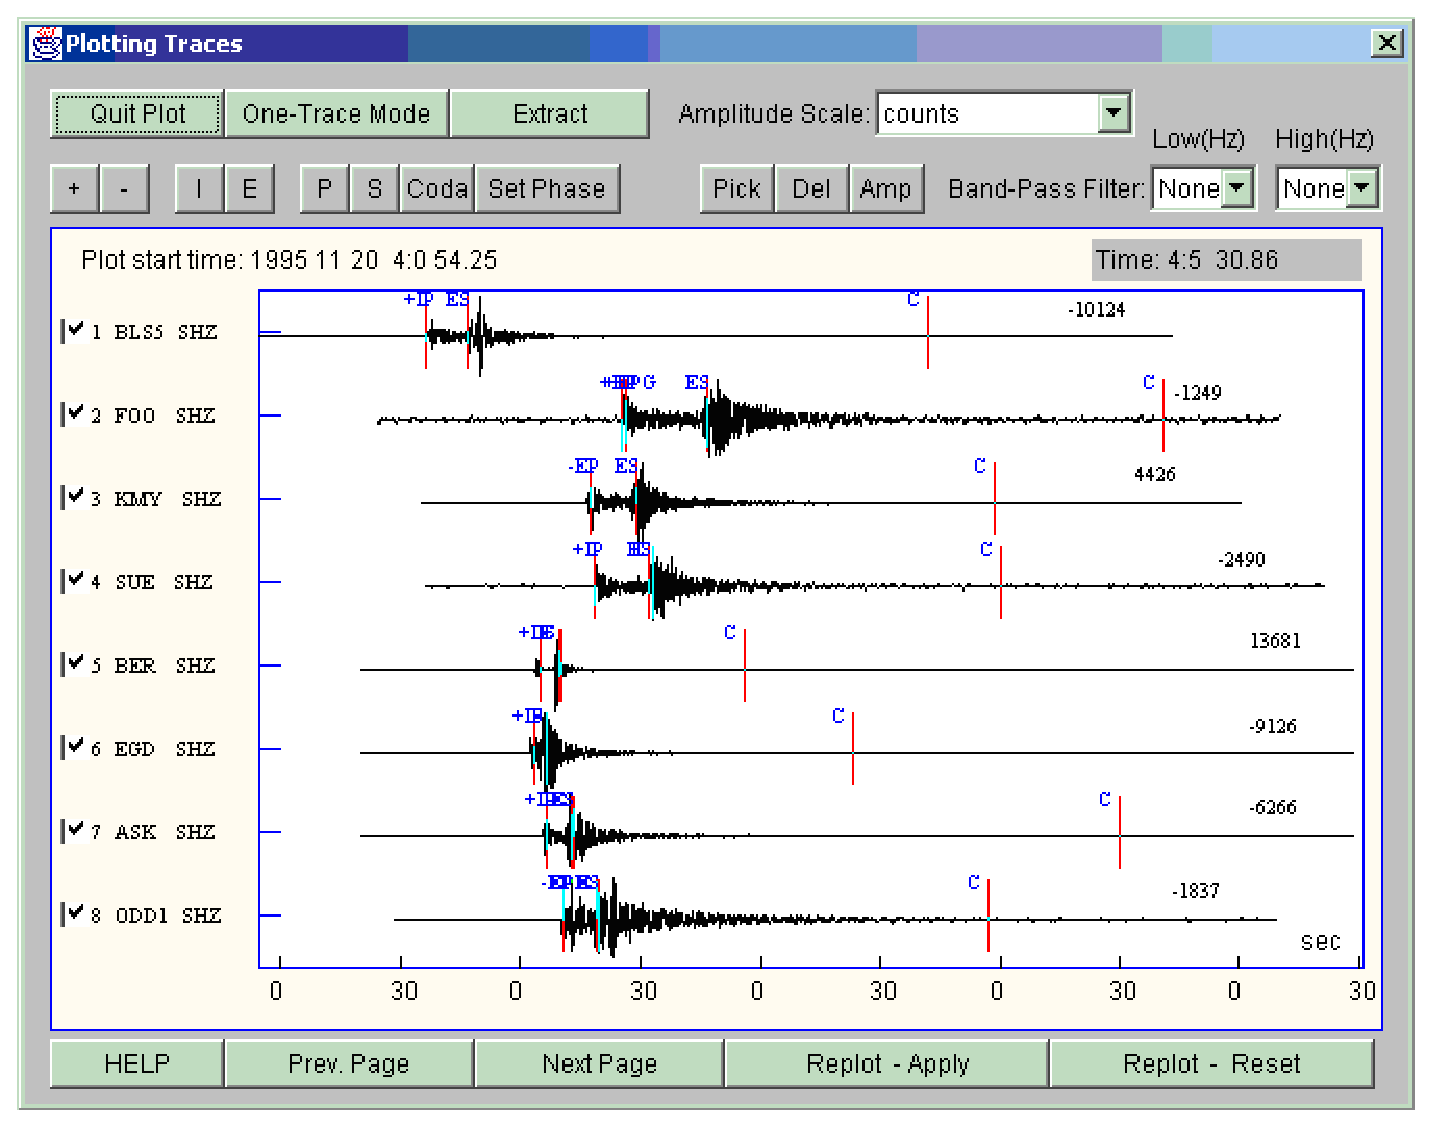
\includegraphics[width=0.9\linewidth]{fig2/fig9}}
\caption{
An example of synthetic seismograms using Bouchon(2),  Herrmann (3) and WKBJ (4). The original seismogram is shown in channel 1. All synthetics are displacement. Also shown are the theoretical travel times calculated by WKBJ. 
}
\label{fig:synthetic}
\end{figure}


